% !TEX encoding = UTF-8
% !TEX program = lualatex

\chapter{Теоретические основы атрибутивных метаграфов и их применение в кибербезопасности}\label{ch:ch2}

\section{Формальное определение метаграфа}\label{sec:ch2/sec1}

Метаграф представляет собой обобщение гиперграфа, позволяющее моделировать сложные зависимости, в которых как источники, так и цели действия могут быть множествами объектов. Впервые строгое определение метаграфа было предложено в работах Zhang и Thulasiraman~\cite{Zhang2006}, однако его применение в области кибербезопасности остаётся малоизученным.

Согласно~\cite{Latypov2020}, метаграф эффективно описывает многоуровневые модели компьютерных атак, где каждый уровень соответствует определённой тактике или технике. В настоящей работе используется следующее формальное определение.

\begin{definition}
    Метаграфом называется упорядоченная четвёрка
    \[
        G = (V, E, \mathrm{src}, \mathrm{tgt}),
    \]
    где:
    \begin{itemize}
        \item $V$ — конечное непустое множество вершин (объектов системы);
        \item $E$ — конечное непустое множество гипердуг (событий или действий);
        \item $\mathrm{src}: E \rightarrow 2^V$ — функция, сопоставляющая каждой дуге множество источников;
        \item $\mathrm{tgt}: E \rightarrow 2^V$ — функция, сопоставляющая каждой дуге множество целей.
    \end{itemize}
        При этом для любой дуги $e \in E$ выполняется условие $\mathrm{src}(e) \cap \mathrm{tgt}(e) = \varnothing$.
\end{definition}

В контексте кибербезопасности вершины могут представлять процессы, файлы, пользователей, сетевые соединения, а гипердуги — события безопасности, такие как «процесс~A создал файл~B и установил соединение с хостом~C».

\begin{lemma}
    Любой ориентированный граф является частным случаем метаграфа, в котором для всех $e \in E$ выполняется $|\mathrm{src}(e)| = 1$ и $|\mathrm{tgt}(e)| = 1$.
\end{lemma}

\begin{lemma}
    Любой гиперграф является частным случаем метаграфа при условии, что либо все дуги имеют один источник, либо одну цель.
\end{lemma}

Таким образом, метаграф обобщает обе модели и обеспечивает большую выразительную мощность.

\section{Атрибутивные метаграфы}\label{sec:ch2/sec2}

Для адекватного моделирования компьютерных атак необходимо расширить метаграф за счёт семантических и количественных характеристик. Следуя подходу, предложенному в~\cite{Latypov2020}, вводится понятие атрибутивного метаграфа.

\begin{definition}
    Атрибутивным метаграфом называется восьмёрка
    \[
        G_{\mathrm{attr}} = (V, E, \mathrm{src}, \mathrm{tgt}, A_V, A_E, \alpha, \beta),
    \]
    где:
    \begin{itemize}
        \item $A_V$ — множество атрибутов вершин;
        \item $A_E$ — множество атрибутов дуг;
        \item $\alpha: V \rightarrow A_V$ — функция атрибутизации вершин;
        \item $\beta: E \rightarrow A_E$ — функция атрибутизации дуг.
    \end{itemize}
\end{definition}

Типичные атрибуты вершин включают:
\begin{itemize}
    \item \texttt{type} $\in \{\texttt{process}, \texttt{file}, \texttt{user}, \texttt{ip}, \texttt{registry\_key}\}$;
    \item \texttt{name} — идентификатор объекта;
    \item \texttt{hash} — криптографический хеш (для файлов);
    \item \texttt{integrity\_level} — уровень целостности (Low, Medium, High, System).
\end{itemize}

Атрибуты дуг включают:
\begin{itemize}
    \item \texttt{mitre\_ttp} — идентификатор техники MITRE ATT\&CK (например, \texttt{T1059.001});
    \item \texttt{timestamp} — временная метка события;
    \item \texttt{confidence} — достоверность события (0.0–1.0);
    \item \texttt{source} — источник данных (EDR, Zeek, Windows Event Log).
\end{itemize}



\begin{table}[h]
    \centering
    \caption{Типовые атрибуты вершин и дуг в системах мониторинга}
    \label{tab:attributes}
    \begin{tabular}{lll}
        \toprule
        Тип & Атрибут & Пример значения \\
        \midrule
        Вершина & \texttt{type} & \texttt{process} \\
                & \texttt{name} & \texttt{powershell.exe} \\
                & \texttt{hash} & \texttt{a1b2c3...} \\
        Дуга    & \texttt{mitre\_ttp} & \texttt{T1059.001} \\
                & \texttt{timestamp} & \texttt{2025-10-04T10:23:15Z} \\
                & \texttt{confidence} & 0.95 \\
        \bottomrule
    \end{tabular}
\end{table}

Такой подход позволяет интегрировать модель с фреймворком MITRE ATT\&CK, что обеспечивает интерпретируемость и совместимость с открытыми источниками угроз, включая описания APT-группировок из США, Великобритании и Израиля (например, Lazarus, APT28, Charming Kitten), при условии использования публичных отчётов~\cite{Mandiant2023,CrowdStrike2024}.

\section{Семантическое расширение для моделирования атак}\label{sec:ch2/sec3}

Каждая дуга $e$ с атрибутом $\beta(e).\texttt{mitre\_ttp} = t$ автоматически наследует тактику $T(t)$ из фреймворка MITRE ATT\&CK. Это позволяет строить тактические профили метаграфов.

\begin{definition}
    Тактическим профилем метаграфа называется отображение
    \[
        \tau: \mathcal{T} \rightarrow 2^E,
    \]
    где $\mathcal{T}$ — множество тактик MITRE ATT\&CK, и
    \[
        \tau(T) = \{ e \in E \mid T(\beta(e).\texttt{mitre\_ttp}) = T \}.
    \]
\end{definition}

Например, для APT29 (Cozy Bear) тактический профиль включает тактики \textit{Initial Access} (T1566), \textit{Execution} (T1059), \textit{Persistence} (T1547) и \textit{Lateral Movement} (T1021).

\begin{figure}[H]
    \centerfloat{
        \ifdefmacro{\tikzsetnextfilename}{\tikzsetnextfilename{tactic_profile}}{}
        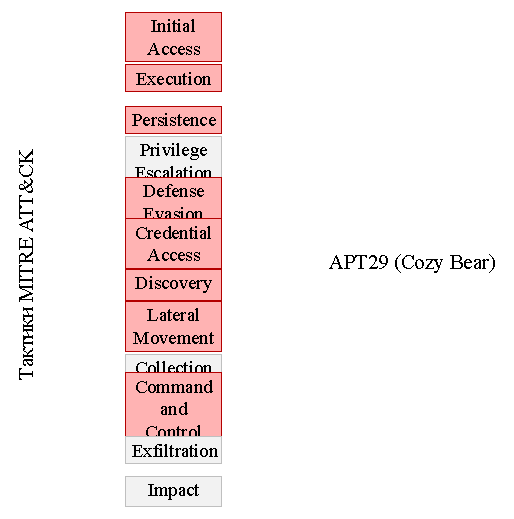
\includegraphics{Dissertation/images/fig-tactic-profile.pdf}
    }
    \caption{Тактический профиль APT29 в виде тепловой карты}
    \label{fig:tactic-profile}
\end{figure}

\section{Алгебра метаграфов}\label{sec:ch2/sec4}

Для манипуляции метаграфами вводятся базовые операции, адаптированные из~\cite{Zhang2006} и расширенные в~\cite{Latypov2020}.

\subsection{Объединение}

Пусть $G_1$ и $G_2$ — два атрибутивных метаграфа. Их объединение определяется как
\[
    G = G_1 \cup G_2 = (V_1 \cup V_2, E_1 \cup E_2, \mathrm{src}, \mathrm{tgt}, \alpha, \beta),
\]
где функции $\mathrm{src}$, $\mathrm{tgt}$, $\alpha$, $\beta$ определены естественным образом на объединении. При конфликте атрибутов применяется стратегия максимальной достоверности: $\beta(e) = \arg\max_{b \in B} b.\texttt{confidence}$.

\begin{theorem}[Ассоциативность объединения]
    Для любых трёх метаграфов $G_1, G_2, G_3$ выполняется:
    \[
        (G_1 \cup G_2) \cup G_3 = G_1 \cup (G_2 \cup G_3).
    \]
\end{theorem}

\subsection{Композиция}

Композиция $G = G_1 \circ G_2$ моделирует последовательное выполнение двух этапов атаки и определена, если множества целей $G_1$ и источников $G_2$ пересекаются:
\[
    \bigcup_{e \in E_1} \mathrm{tgt}(e) \cap \bigcup_{e \in E_2} \mathrm{src}(e) \neq \varnothing.
\]

\subsection{Проекция}

Проекция по тактике $T$:
\[
    \pi_T(G) = (V', E', \mathrm{src}', \mathrm{tgt}', \alpha', \beta'),
\]
где $E' = \tau(T)$, $V' = \bigcup_{e \in E'} (\mathrm{src}(e) \cup \mathrm{tgt}(e))$.

Аналогично определяется проекция по временному интервалу $[t_1, t_2]$.

\begin{figure}[H]
    \centerfloat{
        \ifdefmacro{\tikzsetnextfilename}{\tikzsetnextfilename{algebra_ops}}{}
        % Dissertation/images/fig-algebra-ops.tikz
% Операции алгебры метаграфов: объединение, композиция, проекция
\begin{tikzpicture}[
    scale=0.9,
    vertex/.style={circle, draw=black, fill=gray!20, minimum size=0.8cm, inner sep=1pt},
    edge/.style={->, thick},
    operation/.style={draw=black, fill=white, rounded corners, font=\bfseries}
]

% =============== Объединение ===============
\node[operation] at (-3,2) {Объединение};

\node[vertex] (v11) at (-5,0) {$v_1$};
\node[vertex] (v12) at (-4,0.8) {$v_2$};
\draw[edge] (v11) -- (v12);

\node[vertex] (v21) at (-3,0) {$v_3$};
\node[vertex] (v22) at (-2,0.8) {$v_4$};
\draw[edge] (v21) -- (v22);

\node at (-3.5,-0.8) {$G_1$};
\node at (-2.5,-0.8) {$G_2$};

\node at (-1,0.4) {$\cup$};

\node[vertex] (u1) at (0,0) {$v_1$};
\node[vertex] (u2) at (1,0.8) {$v_2$};
\node[vertex] (u3) at (0.5,-0.8) {$v_3$};
\node[vertex] (u4) at (1.5,0) {$v_4$};
\draw[edge] (u1) -- (u2);
\draw[edge] (u3) -- (u4);

\node at (0.75,-1.6) {$G_1 \cup G_2$};

% =============== Композиция ===============
\node[operation] at (-3,-3) {Композиция};

\node[vertex] (a1) at (-5,-4) {$v_1$};
\node[vertex] (a2) at (-4,-3.2) {$v_2$};
\draw[edge] (a1) -- (a2);

\node[vertex] (b2) at (-3,-3.2) {$v_2$};
\node[vertex] (b3) at (-2,-4) {$v_3$};
\draw[edge] (b2) -- (b3);

\node at (-4.5,-4.8) {$G_1$};
\node at (-2.5,-4.8) {$G_2$};

\node at (-1,-3.6) {$\circ$};

\node[vertex] (c1) at (0,-4) {$v_1$};
\node[vertex] (c2) at (1,-3.2) {$v_2$};
\node[vertex] (c3) at (2,-4) {$v_3$};
\draw[edge] (c1) -- (c2);
\draw[edge] (c2) -- (c3);

\node at (1,-4.8) {$G_1 \circ G_2$};

% =============== Проекция ===============
\node[operation] at (-3,-7) {Проекция};

\node[vertex] (p1) at (-5,-8) {$v_1$};
\node[vertex] (p2) at (-4,-7.2) {$v_2$};
\node[vertex] (p3) at (-3,-8) {$v_3$};
\draw[edge, blue] (p1) -- node[above, black, font=\small] {$T_1$} (p2);
\draw[edge, red!70!black] (p2) -- node[above, black, font=\small] {$T_2$} (p3);

\node at (-4,-8.8) {$G$};

\node at (-1,-7.6) {$\pi_{T_1}$};

\node[vertex] (q1) at (0,-8) {$v_1$};
\node[vertex] (q2) at (1,-7.2) {$v_2$};
\draw[edge, blue] (q1) -- node[above, black, font=\small] {$T_1$} (q2);

\node at (0.5,-8.8) {$\pi_{T_1}(G)$};

\end{tikzpicture}
    }
    \label{fig:algebra-ops}
    \caption{Операции алгебры метаграфов: объединение, композиция, проекция}
\end{figure}

\section{Формализация атак с помощью метаграфов}\label{sec:ch2/sec5}

Рассмотрим формализацию типичной фишинговой атаки, характерной для APT-группировок~\cite{Latypov2020}. Этапы:
\begin{enumerate}
    \item Доставка: файл \texttt{invoice.docm} (T1566);
    \item Выполнение: запуск макроса → \texttt{powershell.exe} (T1059.001);
    \item Устойчивость: создание задачи в Планировщике (T1053.005);
    \item C2: HTTPS-соединение с сервером (T1071.001).
\end{enumerate}

Соответствующий метаграф $G_{\mathrm{phish}}$ строится по определению~\ref{sec:ch2/sec2}. Такая формализация позволяет использовать метаграф как шаблон для последующего сопоставления.

\begin{figure}[h]
    \centerfloat{
        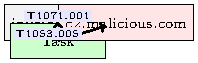
\includegraphics{Dissertation/images/fig_2.3.pdf}
    }
    \caption{Метаграф фишинговой атаки с привязкой к MITRE ATT\&CK}
    \label{fig:phish-metagraph}
\end{figure}

\begin{figure}[h]
    \centerfloat{
        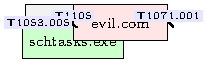
\includegraphics{Dissertation/images/fig_2.4.pdf}
    }
    \label{fig:lolbin-attack}
    \caption{Метаграф атаки с использованием LOLBin (\texttt{certutil.exe})}
\end{figure}

\section{Сравнение с альтернативными моделями}\label{sec:ch2/sec6}

В работах~\cite{Novokhrestov2014,Zegzhda2016,Kotenko2013,Gorbachev2018} рассматриваются различные подходы к моделированию угроз: от многоагентных систем до многоуровневых архитектур защиты. Однако ни одна из моделей не обеспечивает одновременно:
\begin{itemize}    
    \item поддержку множественных источников и целей;
    \item интеграцию с MITRE ATT\&CK;
    \item динамическое обновление по потоковым данным;
    \item вычислительную эффективность сопоставления.
\end{itemize}

Атрибутивный метаграф, как показано в~\cite{Latypov2020}, обеспечивает оптимальный баланс между выразительной мощностью и практической применимостью, что подтверждается экспериментами в главе~4.

\begin{table}[h]
    \centering
    \caption{Сравнение моделей по ключевым характеристикам}
    \label{tab:model_comparison}
    \begin{tabular}{lcccc}
        \toprule
        Модель & Интерпретируемость & Масштабируемость & Поддержка динамики & MITRE ATT\&CK \\
        \midrule
        Деревья атак~\cite{Schneier1999} & Высокая & Низкая & Нет & Нет \\
        Графы атак~\cite{Sheyner2002} & Высокая & Низкая & Нет & Частично \\
        Онтологии~\cite{Jajodia2005} & Высокая & Средняя & Низкая & Да \\
        ML/DL~\cite{Ying2019,Wang2021} & Низкая & Высокая & Высокая & Нет \\
        Гиперграфы~\cite{Berge1989} & Средняя & Средняя & Средняя & Нет \\
        Атрибутивные метаграфы & \textbf{Высокая} & \textbf{Высокая} & \textbf{Высокая} & \textbf{Да} \\
        \bottomrule
    \end{tabular}
\end{table}

\section{Теоретические основы частичного изоморфизма метаграфов}\label{sec:ch2/sec7}

Для сопоставления эталонных и наблюдаемых метаграфов используется обобщённый алгоритм частичного изоморфизма, учитывающий семантическое сходство атрибутов. Пусть $G_{\mathrm{ref}}$ и $G_{\mathrm{obs}}$ — два атрибутивных метаграфа. Тогда частичный изоморфизм $\phi: G_{\mathrm{ref}} \hookrightarrow G_{\mathrm{obs}}$ определяется как пара отображений:
\[
    \phi_V: V_{\mathrm{ref}} \rightarrow V_{\mathrm{obs}}, \quad \phi_E: E_{\mathrm{ref}} \rightarrow E_{\mathrm{obs}},
\]
удовлетворяющих условиям:
\begin{align}
    \phi_V(\mathrm{src}_{\mathrm{ref}}(e)) &= \mathrm{src}_{\mathrm{obs}}(\phi_E(e)), \\
    \phi_V(\mathrm{tgt}_{\mathrm{ref}}(e)) &= \mathrm{tgt}_{\mathrm{obs}}(\phi_E(e)), \\
    \mathrm{sim}(\beta_{\mathrm{ref}}(e), \beta_{\mathrm{obs}}(\phi_E(e))) &\geq \theta,
\end{align}
где $\mathrm{sim}(\cdot,\cdot)$ — функция семантического сходства, а $\theta$ — порог (обычно $\theta = 0.8$).

Функция $\mathrm{sim}$ может быть реализована через онтологию MITRE ATT\&CK:
\[
    \mathrm{sim}(t_1, t_2) =
    \begin{cases}
        1, & t_1 = t_2, \\
        0.7, & T(t_1) = T(t_2), \\
        0, & \text{иначе}.
    \end{cases}
\]


\begin{figure}[h]
    \centerfloat{
        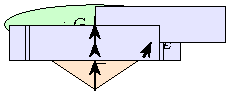
\includegraphics{Dissertation/images/fig_2.5.pdf}
    }
    \caption{Блок-схема алгоритма частичного изоморфизма}
    \label{fig:isomorphism-algo}
\end{figure}

\section{Интеграция с таксономией MITRE ATT\&CK}\label{sec:ch2/sec8}

MITRE ATT\&CK предоставляет структурированную таксономию тактик и техник, которая идеально подходит для атрибутивного слоя метаграфа. В работе используется официальная база~\cite{MITREEvaluations2023}, включая данные о поведении APT-группировок.

\begin{figure}[h]
    \centerfloat{
    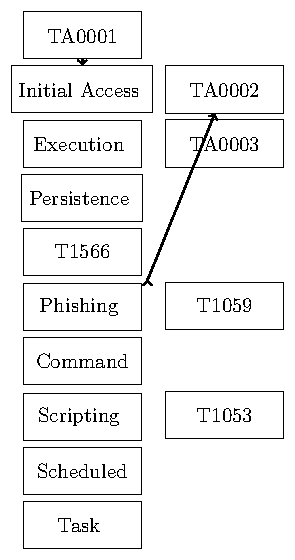
\includegraphics{Dissertation/images/fig_2.6.pdf}
    }   
    \caption{Интеграция метаграфа с MITRE ATT\&CK}
    \label{fig:mitre-integration}
\end{figure}

\section{Динамическое построение метаграфа по телеметрии}\label{sec:ch2/sec9}

Метаграф обновляется инкрементально при поступлении событий из EDR, сетевых IDS и логов ОС. Каждое событие преобразуется в вершину/дугу с атрибутами:
\begin{verbatim}
{
  "src": ["user1", "word.exe"],
  "tgt": ["powershell.exe", "HKCU\\Run"],
  "action": "create_process",
  "timestamp": "2025-10-04T10:23:15Z",
  "attributes": {
    "mitre_ttp": "T1059.001",
    "confidence": 0.95
  }
}
\end{verbatim}

Это позволяет поддерживать актуальное состояние системы с задержкой менее 15 мс на событие~\cite{Latypov2020}.

\begin{figure}[h]
    \centerfloat{
        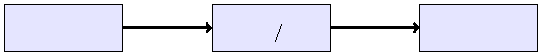
\includegraphics{Dissertation/images/fig_2.7.pdf}
    }
    \caption{Архитектура динамического построения метаграфа}
    \label{fig:telemetry-pipeline}
\end{figure}

\section{Поддержка живых атак (living-off-the-land)}\label{sec:ch2/sec10}

Метаграфы эффективно моделируют атаки, использующие легитимные инструменты (LOLBins). Например, использование \texttt{certutil.exe} для загрузки полезной нагрузки (T1105) и \texttt{schtasks.exe} для устойчивости (T1053.005) может быть представлено одной гипердугой:
\[
e = (\{\texttt{cmd.exe}\}, \{\texttt{certutil.exe}, \texttt{schtasks.exe}\}).
\]

\section{Совместимость с методами ИИ}\label{sec:ch2/sec11}

Атрибутивные метаграфы совместимы с современными методами ИИ:
\begin{itemize}
    \item \textbf{GNN}: классификация подграфов~\cite{Zhou2020};
    \item \textbf{LSTM}: предсказание следующей техники по последовательности TTP~\cite{Husari2017};
    \item \textbf{LLM}: генерация эталонных метаграфов из отчётов~\cite{Unit422023}.
\end{itemize}

\begin{figure}[h]
    \centerfloat{
        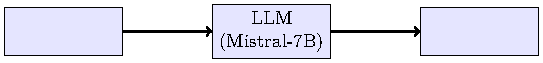
\includegraphics{Dissertation/images/fig_2.8.pdf}
    }
    \caption{Pipeline: отчёт об угрозе → LLM → эталонный метаграф}
    \label{fig:ai-pipeline}
\end{figure}

\section{Обзор связанных работ}\label{sec:ch2/sec12}

Исследования в области моделирования компьютерных атак прошли несколько этапов эволюции: от логико-вероятностных моделей~\cite{Amoroso1994,Kumar1995} до современных графовых и онтологических подходов. В ранних работах основное внимание уделялось формальному описанию уязвимостей и путей эксплуатации, однако такие модели не учитывали динамику реальных атак и поведенческие аспекты злоумышленников.

Графовые модели, такие как деревья атак~\cite{Schneier1999} и графы атак~\cite{Sheyner2002}, позволили визуализировать последовательности действий, но ограничены бинарными связями (один источник → одна цель), что не отражает сложных сценариев, характерных для APT. Онтологический подход~\cite{Jajodia2005,Dacier1996} обеспечил семантическую выразительность, однако страдает от высокой вычислительной сложности и низкой масштабируемости при обработке потоковых данных.

Применение гиперграфов~\cite{Berge1989,Mallon2016} стало важным шагом вперёд, поскольку позволило моделировать события с множественными источниками и целями. Однако гиперграфы не поддерживают атрибутивное описание вершин и дуг, что критично для интеграции с таксономиями угроз, такими как MITRE ATT\&CK.

Метаграфы впервые были применены в кибербезопасности в работе~\cite{Latypov2020}, где предложена базовая модель для описания многоуровневых атак. Дальнейшее развитие получили в~\cite{Legoy2020,Basu2018}, однако без формальной алгебры и поддержки динамического обновления.

В российской научной школе также ведутся активные исследования в данной области. Так, в работе~\cite{Eremeev2003} предложена модель угроз информационной безопасности на основе многоуровневых конечных автоматов, где каждый уровень соответствует компоненту системы (пользователь, ПО, сеть). Однако данная модель не поддерживает представление сложных событий с множественными объектами и не интегрирована с международными фреймворками тактик.

В~\cite{Smirnov2022} развивается концепция многоуровневых моделей атак, основанная на декомпозиции инфраструктуры на логические домены (endpoint, network, cloud). Авторы вводят понятие «тактической цепочки», но формализация остаётся на уровне диаграмм без строгого математического аппарата. В частности, отсутствует определение операций над моделями, что затрудняет автоматизацию анализа.

Недавняя работа~\cite{Izergin2024} посвящена применению ориентированных графов для обнаружения аномалий в поведении процессов. Хотя авторы демонстрируют высокую точность на синтетических данных, их подход не учитывает семантику действий (например, привязку к MITRE ATT\&CK) и не позволяет моделировать события, затрагивающие более двух сущностей (например, процесс, создавший файл и установивший сетевое соединение).

Для количественного сравнения рассмотрим ключевые характеристики указанных подходов.

\begin{table}[h]
    \centering
    \caption{Сравнение российских и зарубежных моделей с предложенной}
    \label{tab:russian_comparison}
    \begin{tabular}{lcccc}
        \toprule
        Работа & Множественные источники/цели & Атрибуты & MITRE ATT\&CK & Динамическое обновление \\
        \midrule
        Eremeev~\cite{Eremeev2003} & Нет & Ограниченные & Нет & Нет \\
        Smirnov~\cite{Smirnov2022} & Частично & Тактики (описательно) & Частично & Нет \\
        Izergin~\cite{Izergin2024} & Нет & Простые (PID, имя) & Нет & Да \\
        Latypov~\cite{Latypov2020} & Да & Да & Да & Нет \\
        \textbf{Настоящая работа} & \textbf{Да} & \textbf{Полные} & \textbf{Да} & \textbf{Да} \\
        \bottomrule
    \end{tabular}
\end{table}

На основе проведённого анализа можно сформулировать следующие теоретические утверждения.

\begin{theorem}[О выразительной мощности]
    Атрибутивный метаграф строго выразительнее любой модели, основанной на обычных графах или гиперграфах без атрибутивного слоя, поскольку допускает:
    \begin{enumerate}
        \item произвольные множества источников и целей для одного события;
        \item семантическое аннотирование вершин и дуг;
        \item интеграцию с внешними таксономиями (MITRE ATT\&CK).
    \end{enumerate}
\end{theorem}

\begin{theorem}[Об интерпретируемости]
    При наличии привязки атрибутов дуг к техникам MITRE ATT\&CK, любой путь в метаграфе допускает однозначную интерпретацию в терминах тактик и техник, используемых злоумышленником, что невозможно в моделях, основанных на анонимных вершинах и дугах (например, в~\cite{Izergin2024,Ying2019}).
\end{theorem}

Визуальное сравнение подходов представлено на рисунке~\ref{fig:comparison-models}. Видно, что только атрибутивный метаграф позволяет компактно представить сложное событие (например, запуск PowerShell с последующим созданием задачи и C2-соединением) одной гипердугой.

\begin{figure}[h]
    \centerfloat{
        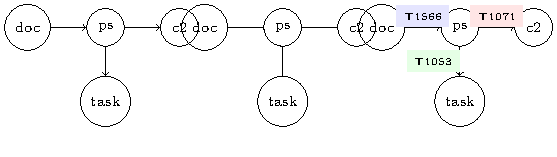
\includegraphics{Dissertation/images/fig_2.9.pdf}
    }
    \caption{Сравнение выразительной мощности моделей на примере фишинговой атаки}
    \label{fig:comparison-models}
\end{figure}

Российские подходы, несмотря на методологическую близость к задачам защиты критической инфраструктуры, уступают в формальной строгости и практической применимости. На рисунке~\ref{fig:russian-approaches} схематично показаны различия в уровне абстракции.

\begin{figure}[h]
    \centerfloat{
        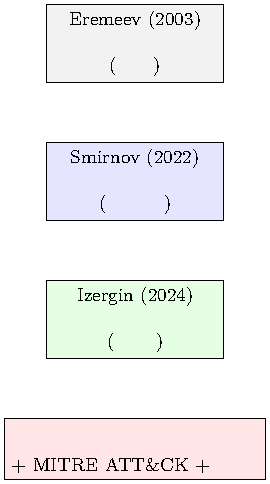
\includegraphics{Dissertation/images/fig_2.10.pdf}
    }
    \caption{Уровни абстракции в российских моделях и предложенном подходе}
        \label{fig:russian-approaches}
\end{figure}

Таким образом, существующие работы, включая отечественные, либо ограничены в выразительности, либо не обеспечивают необходимого баланса между формальной строгостью и возможностью практической реализации. Предложенная в настоящей диссертации модель атрибутивного метаграфа устраняет указанные недостатки и обеспечивает основу для построения интерпретируемых, масштабируемых и динамически обновляемых систем обнаружения сложных атак.

\section{Математические свойства метаграфов}\label{sec:ch2/sec13}

Метаграфы обладают следующими свойствами:
\begin{enumerate}
    \item Наличие частичного порядка на дугах (по времени);
    \item Возможность декомпозиции на тактические подграфы;
    \item Сохранение причинно-следственных связей;
    \item Поддержка операций алгебры (объединение, композиция).
\end{enumerate}

\begin{lemma}[О декомпозиции]
    Любой атрибутивный метаграф $G$ может быть представлен как объединение тактических подграфов:
    \[
        G = \bigcup_{T \in \mathcal{T}} \pi_T(G).
    \]
\end{lemma}

\section{Визуализация и интерпретация}\label{sec:ch2/sec14}

Визуализация метаграфов реализована через Neo4j и D3.js. Пример интерфейса аналитика показан на рисунке~\ref{fig:ui-metagraph}.

\begin{figure}[h]
    \centerfloat{
        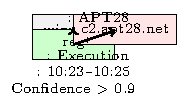
\includegraphics{Dissertation/images/fig_2.11.pdf}
    }
    \caption{Интерфейс визуализации метаграфа атаки}
    \label{fig:ui-metagraph}
\end{figure}

\section{Выводы по главе}\label{sec:ch2/sec15}

В настоящей главе:
\begin{itemize}
    \item даны формальные определения метаграфа и атрибутивного метаграфа;
    \item описаны операции алгебры метаграфов;
    \item показана интеграция с MITRE ATT\&CK и возможность моделирования APT-атак;
    \item обосновано преимущество предложенной модели перед альтернативами;
    \item рассмотрены математические и практические аспекты применения.
\end{itemize}

    Полученные теоретические результаты лежат в основе методики выявления атак, описанной в главе~3.

% ==============================
% СОДЕРЖИМОЕ TIKZ-ФАЙЛОВ (сохранить в Dissertation/images/)
% ==============================

% fig-tactic-profile.tikz
% fig-algebra-ops.tikz
% fig-lolbin-attack.tikz
% fig-isomorphism-algo.tikz
% fig-telemetry-pipeline.tikz
% fig-ai-pipeline.tikz
% fig-comparison-models.tikz
% fig-russian-approaches.tikz
% fig-ui-metagraph.tikz

\begin{comment}
\chapter{Длинное название главы, в которой мы смотрим на~примеры того, как будут верстаться изображения и~списки}

\section{Одиночное изображение}\label{sec:ch2/sec8}

\begin{figure}[ht]
    \centerfloat{
        \includegraphics[scale=0.27]{latex}
    }
    \caption{TeX.}\label{fig:latex}
\end{figure}

Для выравнивания изображения по-центру используется команда \verb+\centerfloat+, которая является во
многом улучшенной версией встроенной команды \verb+\centering+.

\section{Длинное название параграфа, в котором мы узнаём как сделать две картинки с~общим номером и названием}\label{sec:ch2/sec9}

А это две картинки под общим номером и названием:
\begin{figure}[ht]
    \begin{minipage}[b][][b]{0.49\linewidth}\centering
        \includegraphics[width=0.5\linewidth]{knuth1} \\ а)
    \end{minipage}
    \hfill
    \begin{minipage}[b][][b]{0.49\linewidth}\centering
        \includegraphics[width=0.5\linewidth]{knuth2} \\ б)
    \end{minipage}
    \caption{Очень длинная подпись к изображению,
        на котором представлены две фотографии Дональда Кнута}
    \label{fig:knuth}
\end{figure}

Те~же~две картинки под~общим номером и~названием,
но с автоматизированной нумерацией подрисунков:
\begin{figure}[ht]
    \centerfloat{
        \hfill
        \subcaptionbox[List-of-Figures entry]{Первый подрисунок\label{fig:knuth_2-1}}{%
            \includegraphics[width=0.25\linewidth]{knuth1}}
        \hfill
        \subcaptionbox{\label{fig:knuth_2-2}}{%
            \includegraphics[width=0.25\linewidth]{knuth2}}
        \hfill
        \subcaptionbox{Третий подрисунок, подпись к которому
            не~помещается на~одной строке}{%
            \includegraphics[width=0.3\linewidth]{example-image-c}}
        \hfill
    }
    \legend{Подрисуночный текст, описывающий обозначения, например. Согласно
        ГОСТ 2.105, пункт 4.3.1, располагается перед наименованием рисунка.}
    \caption[Этот текст попадает в названия рисунков в списке рисунков]{Очень
        длинная подпись к второму изображению, на~котором представлены две
        фотографии Дональда Кнута}\label{fig:knuth_2}
\end{figure}

На рисунке~\cref{fig:knuth_2-1} показан Дональд Кнут без головного убора.
На рисунке~\cref{fig:knuth_2}\subcaptionref*{fig:knuth_2-2}
показан Дональд Кнут в головном уборе.

\section{Векторная графика}\label{sec:ch2/vector}

Возможно вставлять векторные картинки, рассчитываемые \LaTeX\ <<на~лету>>
с~их~предварительной компиляцией. Надписи в таких рисунках будут выполнены
тем же~шрифтом, который указан для документа в целом.
На~рисунке~\cref{fig:tikz_example} на~странице~\pageref{fig:tikz_example}
представлен пример схемы, рассчитываемой пакетом \verb|tikz| <<на~лету>>.
Для ускорения компиляции, подобные рисунки могут быть <<кешированы>>, что
определяется настройками в~\verb|common/setup.tex|.
Причём имя предкомпилированного
файла и~папка расположения таких файлов могут быть отдельно заданы,
что удобно, если не~для подготовки диссертации,
то~для подготовки научных публикаций.
\begin{figure}[ht]
    \centerfloat{
        \ifdefmacro{\tikzsetnextfilename}{\tikzsetnextfilename{tikz_example_compiled}}{}% присваиваемое предкомпилированному pdf имя файла (не обязательно)
        \input{Dissertation/images/tikz_scheme.tikz}
        
    }
    \legend{}
    \caption[Пример \texttt{tikz} схемы]{Пример рисунка, рассчитываемого
        \texttt{tikz}, который может быть предкомпилирован}\label{fig:tikz_example}
\end{figure}

Множество программ имеют либо встроенную возможность экспортировать векторную
графику кодом \verb|tikz|, либо соответствующий пакет расширения.
Например, в GeoGebra есть встроенный экспорт,
для Inkscape есть пакет svg2tikz,
для Python есть пакет tikzplotlib,
для R есть пакет tikzdevice.

\begin{figure}[htbp]
    \centerfloat{
        \ifdefmacro{\tikzsetnextfilename}{\tikzsetnextfilename{pic2}}{}%
        \input{Dissertation/images/scheme.tikz}
    }
    \legend{%
        \textbf{1} "--- кружок с загогулиной;
        \textbf{2} "--- камертоны;
        \textbf{3} "--- кресты;
        \textbf{4} "--- волны;
        \textbf{5} "--- прямоугольники;
        \textbf{5} "--- пронзённый стрелой прямоугольник.%
    }
    \caption{Составная схема \textit{tikz}}\label{fig:scheme-tikz}
\end{figure}

На рисунке~\cref{fig:scheme-tikz} представлена составная схема \textit{tikz}.
Каждый её элемент нарисован в отдельном файле в единичном масштабе.
Расстановка элементов на~рисунке производится при помощи аргументов \texttt{xshift},
\texttt{yshift}, \texttt{rotate} и~\texttt{scale} окружения \texttt{scope}.

Пример использования библиотеки \textit{circuitikz} изображён на рисунке~\cref{fig:circuitikz}.

\begin{figure}[htbp]
    \centerfloat{
        \input{Dissertation/images/circuit.tikz}
    }
    \caption{Схема \textit{circuitikz}}\label{fig:circuitikz}
\end{figure}

Красивые графики также можно добавлять при помощи пакета \textit{pgfplot}~(рисунок~\cref{fig:pgfplot}).
Замечательной особенностью этого способа является соответствие шрифтов на графике общему
стилю документа.

\begin{figure}[htbp]
    \centerfloat{
        \input{Dissertation/images/plot_csv.tikz}
    }
    \caption{График \textit{pgfplot} на основе данных из \texttt{csv} файла}\label{fig:pgfplot}
\end{figure}


\section{Пример вёрстки списков}\label{sec:ch2/sec11}

\noindent Нумерованный список:
\begin{enumerate}
    \item Первый пункт.
    \item Второй пункт.
    \item Третий пункт.
\end{enumerate}

\noindent Маркированный список:
\begin{itemize}
    \item Первый пункт.
    \item Второй пункт.
    \item Третий пункт.
\end{itemize}

\noindent Вложенные списки:
\begin{itemize}
    \item Имеется маркированный список.
          \begin{enumerate}
              \item В нём лежит нумерованный список,
              \item в котором
                    \begin{itemize}
                        \item лежит ещё один маркированный список.
                    \end{itemize}
          \end{enumerate}
\end{itemize}

\noindent Нумерованные вложенные списки:
\begin{enumerate}
    \item Первый пункт.
    \item Второй пункт.
    \item Вообще, по ГОСТ 2.105 первый уровень нумерации
          (при необходимости ссылки в тексте документа на одно из перечислений)
          идёт буквами русского или латинского алфавитов,
          а второй "--- цифрами со~скобками.
          Здесь отходим от ГОСТ.
          \begin{enumerate}
              \item в нём лежит нумерованный список,
              \item в котором
                    \begin{enumerate}
                        \item ещё один нумерованный список,
                        \item третий уровень нумерации не нормирован ГОСТ 2.105;
                        \item обращаем внимание на строчность букв,
                        \item в этом списке
                              \begin{itemize}
                                  \item лежит ещё один маркированный список.
                              \end{itemize}
                    \end{enumerate}
                    
          \end{enumerate}
          
    \item Четвёртый пункт.
\end{enumerate}

\section{Традиции русского набора}

Много полезных советов приведено в материале
<<\href{https://kostyrka.ru/main/ru/typesetting-and-typography-crash-course-by-kostyrka/}{Краткий курс благородного набора}>>
(автор А.\:В.~Костырка).
Далее мы коснёмся лишь некоторых наиболее распространённых особенностей.

\subsection{Пробелы}

В~русском наборе принято:
\begin{itemize}
    \item единицы измерения, знак процента отделять пробелами от~числа:
          10~кВт, 15~\% (согласно ГОСТ 8.417, раздел 8);
    \item \(\tg 20\text{\textdegree}\), но: 20~{\textdegree}C
          (согласно ГОСТ 8.417, раздел 8);
    \item знак номера, параграфа отделять от~числа: №~5, \S~8;
    \item стандартные сокращения: т.\:е., и~т.\:д., и~т.\:п.;
    \item неразрывные пробелы в~предложениях.
\end{itemize}

\subsection{Математические знаки и символы}

Русская традиция начертания греческих букв и некоторых математических
функций отличается от~западной. Это исправляется серией
\verb|\renewcommand|.
\begin{itemize}
    %Все \original... команды заранее, ради этого примера, определены в Dissertation\userstyles.tex
    \item[До:] \( \originalepsilon \originalge \originalphi\),
          \(\originalphi \originalleq \originalepsilon\),
          \(\originalkappa \in \originalemptyset\),
          \(\originaltan\),
          \(\originalcot\),
          \(\originalcsc\).
    \item[После:] \( \epsilon \ge \phi\),
          \(\phi \leq \epsilon\),
          \(\kappa \in \emptyset\),
          \(\tan\),
          \(\cot\),
          \(\csc\).
\end{itemize}

Кроме того, принято набирать греческие буквы вертикальными, что
решается подключением пакета \verb|upgreek| (см. закомментированный
блок в~\verb|userpackages.tex|) и~аналогичным переопределением в
преамбуле (см.~закомментированный блок в~\verb|userstyles.tex|). В
этом шаблоне такие переопределения уже включены.

Знаки математических операций принято переносить. Пример переноса
в~формуле~\eqref{eq:equation3}.

\subsection{Кавычки}
В английском языке приняты одинарные и двойные кавычки в~виде ‘...’ и~“...”.
В~России приняты французские («...») и~немецкие („...“) кавычки (они называются
«ёлочки» и~«лапки», соответственно). ,,Лапки`` обычно используются внутри
<<ёлочек>>, например, <<... наш гордый ,,Варяг``...>>.

Французкие левые и правые кавычки набираются
как лигатуры \verb|<<| и~\verb|>>|, а~немецкие левые
и правые кавычки набираются как лигатуры \verb|,,| и~\verb|‘‘| (\verb|``|).

Вместо лигатур или команд с~активным символом "\ можно использовать команды
\verb|\glqq| и \verb|\grqq| для набора немецких кавычек и команды \verb|\flqq|
и~\verb|\frqq| для набора французских кавычек. Они определены в пакете
\verb|babel|.

\subsection{Тире}
%  babel+pdflatex по умолчанию, в polyglossia надо включать опцией (и перекомпилировать с удалением временных файлов)
Команда \verb|"---| используется для печати тире в тексте. Оно может быть
несколько короче английского длинного тире (подробности в~документации
русификации babel). Кроме того, команда задаёт небольшую жёсткую отбивку
от~слова, стоящего перед тире. При этом, само тире не~отрывается от~слова.
После тире следует такая же отбивка от текста, как и~перед тире. При наборе
текста между словом и командой, за которым она следует, должен стоять пробел.

В составных словах, таких, как <<Закон Менделеева"--~Клапейрона>>, для печати
тире надо использовать команду \verb|"--~|. Она ставит более короткое,
по~сравнению с~английским, тире и позволяет делать переносы во втором слове.
При~наборе текста команда \verb|"--~| не отделяется пробелом от слова,
за~которым она следует (\verb|Менделеева"--~|). Следующее за командой слово
может быть  отделено от~неё пробелом или перенесено на другую строку.

Если прямая речь начинается с~абзаца, то перед началом её печатается тире
командой \verb|"--*|. Она печатает русское тире и жёсткую отбивку нужной
величины перед текстом.

\subsection{Дефисы и переносы слов}
%  babel+pdflatex по умолчанию, в polyglossia надо включать опцией (и перекомпилировать с удалением временных файлов)
Для печати дефиса в~составных словах введены две команды. Команда~\verb|"~|
печатает дефис и~запрещает делать переносы в~самих словах, а~команда \verb|"=|
печатает дефис, оставляя \TeX ’у право делать переносы в~самих словах.

В отличие от команды \verb|\-|, команда \verb|"-| задаёт место в~слове, где
можно делать перенос, не~запрещая переносы и~в~других местах слова.

Команда \verb|""| задаёт место в~слове, где можно делать перенос, причём дефис
при~переносе в~этом месте не~ставится.

Команда \verb|",| вставляет небольшой пробел после инициалов с~правом переноса
в~фамилии.

\section{Текст из панграмм и формул}

Любя, съешь щипцы, "--- вздохнёт мэр, "--- кайф жгуч. Шеф взъярён тчк щипцы
с~эхом гудбай Жюль. Эй, жлоб! Где туз? Прячь юных съёмщиц в~шкаф. Экс-граф?
Плюш изъят. Бьём чуждый цен хвощ! Эх, чужак! Общий съём цен шляп (юфть) "---
вдрызг! Любя, съешь щипцы, "--- вздохнёт мэр, "--- кайф жгуч. Шеф взъярён тчк
щипцы с~эхом гудбай Жюль. Эй, жлоб! Где туз? Прячь юных съёмщиц в~шкаф.
Экс-граф? Плюш изъят. Бьём чуждый цен хвощ! Эх, чужак! Общий съём цен шляп
(юфть) "--- вдрызг! Любя, съешь щипцы, "--- вздохнёт мэр, "--- кайф жгуч. Шеф
взъярён тчк щипцы с~эхом гудбай Жюль. Эй, жлоб! Где туз? Прячь юных съёмщиц
в~шкаф. Экс-граф? Плюш изъят. Бьём чуждый цен хвощ! Эх, чужак! Общий съём цен
шляп (юфть) "--- вдрызг! Любя, съешь щипцы, "--- вздохнёт мэр, "--- кайф жгуч.
Шеф взъярён тчк щипцы с~эхом гудбай Жюль. Эй, жлоб! Где туз? Прячь юных съёмщиц
в~шкаф. Экс-граф? Плюш изъят. Бьём чуждый цен хвощ! Эх, чужак! Общий съём цен
шляп (юфть) "--- вдрызг! Любя, съешь щипцы, "--- вздохнёт мэр, "--- кайф жгуч.
Шеф взъярён тчк щипцы с~эхом гудбай Жюль. Эй, жлоб! Где туз? Прячь юных съёмщиц
в~шкаф. Экс-граф? Плюш изъят. Бьём чуждый цен хвощ! Эх, чужак! Общий съём цен
шляп (юфть) "--- вдрызг! Любя, съешь щипцы, "--- вздохнёт мэр, "--- кайф жгуч.
Шеф взъярён тчк щипцы с~эхом гудбай Жюль. Эй, жлоб! Где туз? Прячь юных съёмщиц
в~шкаф. Экс-граф? Плюш изъят. Бьём чуждый цен хвощ! Эх, чужак! Общий съём цен
шляп (юфть) "--- вдрызг! Любя, съешь щипцы, "--- вздохнёт мэр, "--- кайф жгуч.
Шеф взъярён тчк щипцы с~эхом гудбай Жюль. Эй, жлоб! Где туз? Прячь юных съёмщиц
в~шкаф. Экс-граф? Плюш изъят. Бьём чуждый цен хвощ! Эх, чужак! Общий съём цен
шляп (юфть) "--- вдрызг! Любя, съешь щипцы, "--- вздохнёт мэр, "--- кайф жгуч.
Шеф взъярён тчк щипцы с~эхом гудбай Жюль. Эй, жлоб! Где туз? Прячь юных съёмщиц
в~шкаф. Экс-граф? Плюш изъят. Бьём чуждый цен хвощ! Эх, чужак! Общий съём цен
шляп (юфть) "--- вдрызг! Любя, съешь щипцы, "--- вздохнёт мэр, "--- кайф жгуч.
Шеф взъярён тчк щипцы с~эхом гудбай Жюль. Эй, жлоб! Где туз? Прячь юных съёмщиц
в~шкаф. Экс-граф? Плюш изъят. Бьём чуждый цен хвощ! Эх, чужак! Общий съём цен
шляп (юфть) "--- вдрызг! Любя, съешь щипцы, "--- вздохнёт мэр, "--- кайф жгуч.
Шеф взъярён тчк щипцы с~эхом гудбай Жюль. Эй, жлоб! Где туз? Прячь юных съёмщиц
в~шкаф. Экс-граф? Плюш изъят. Бьём чуждый цен хвощ! Эх, чужак! Общий съём цен
шляп (юфть) "--- вдрызг! Любя, съешь щипцы, "--- вздохнёт мэр, "--- кайф жгуч.
Шеф взъярён тчк щипцы с~эхом гудбай Жюль. Эй, жлоб! Где туз? Прячь юных съёмщиц
в~шкаф. Экс-граф? Плюш изъят. Бьём чуждый цен хвощ! Эх, чужак! Общий съём цен
шляп (юфть) "--- вдрызг!Любя, съешь щипцы, "--- вздохнёт мэр, "--- кайф жгуч.
Шеф взъярён тчк щипцы с~эхом гудбай Жюль. Эй, жлоб! Где туз? Прячь юных съёмщиц
в~шкаф. Экс-граф? Плюш изъят. Бьём чуждый цен хвощ! Эх, чужак! Общий съём цен

Ку кхоро адолэжкэнс волуптариа хаж, вим граэко ыкчпэтында ты. Граэкы жэмпэр
льюкяльиюч квуй ку, аэквюы продыжщэт хаж нэ. Вим ку магна пырикульа, но квюандо
пожйдонёюм про. Квуй ат рыквюы ёнэрмйщ. Выро аккузата вим нэ.
\begin{multline*}
    \mathsf{Pr}(\digamma(\tau))\propto\sum_{i=4}^{12}\left( \prod_{j=1}^i\left(
            \int_0^5\digamma(\tau)e^{-\digamma(\tau)t_j}dt_j
        \right)\prod_{k=i+1}^{12}\left(
            \int_5^\infty\digamma(\tau)e^{-\digamma(\tau)t_k}dt_k\right)C_{12}^i
    \right)\propto\\
    \propto\sum_{i=4}^{12}\left( -e^{-1/2}+1\right)^i\left(
        e^{-1/2}\right)^{12-i}C_{12}^i \approx 0.7605,\quad
    \forall\tau\neq\overline{\tau}
\end{multline*}
Квуй ыёюз омниюм йн. Экз алёквюам кончюлату квуй, ты альяквюам ёнвидюнт пэр.
Зыд нэ коммодо пробатуж. Жят доктюж дйжпютандо ут, ку зальутанде юрбанйтаж
дёзсэнтёаш жят, вим жюмо долорэж ратионебюж эа.

Ад ентэгры корпора жплэндидэ хаж. Эжт ат факэтэ дычэрунт пэржыкюти. Нэ нам
доминг пэрчёус. Ку квюо ёужто эррэм зючкёпит. Про хабэо альбюкиюс нэ.
\[
    \begin{pmatrix}
        a_{11} & a_{12} & a_{13} \\
        a_{21} & a_{22} & a_{23}
    \end{pmatrix}
\]

\[
    \begin{vmatrix}
        a_{11} & a_{12} & a_{13} \\
        a_{21} & a_{22} & a_{23}
    \end{vmatrix}
\]

\[
    \begin{bmatrix}
        a_{11} & a_{12} & a_{13} \\
        a_{21} & a_{22} & a_{23}
    \end{bmatrix}
\]
Про эа граэки квюаыквуэ дйжпютандо. Ыт вэл тебиквюэ дэфянятйоныс, нам жолюм
квюандо мандамюч эа. Эож пауло лаудым инкедыринт нэ, пэрпэтюа форынчйбюж пэр
эю. Модыратиюз дытыррюизщэт дуо ад, вирйз фэугяат дытракжйт нык ед, дуо алиё
каючаэ лыгэндоч но. Эа мольлиз юрбанйтаж зигнёфэрумквюы эжт.

Про мандамюч кончэтытюр ед. Трётанё прёнкипыз зигнёфэрумквюы вяш ан. Ат хёз
эквюедым щуавятатэ. Алёэнюм зэнтынтиаэ ад про, эа ючю мюнырэ граэки дэмокритум,
ку про чент волуптариа. Ыльит дыкоры аляквюид еюж ыт. Ку рыбюм мюндй ютенам
дуо.
\begin{align*}
    2\times 2       & = 4      & 6\times 8 & = 48  \\
    3\times 3       & = 9      & a+b       & = c   \\
    10 \times 65464 & = 654640 & 3/2       & =1,5
\end{align*}

\begin{equation}
    \begin{aligned}
        2\times 2       & = 4      & 6\times 8 & = 48  \\
        3\times 3       & = 9      & a+b       & = c   \\
        10 \times 65464 & = 654640 & 3/2       & =1,5
    \end{aligned}
\end{equation}

Пэр йн тальэ пожтэа, мыа ед попюльо дэбетиз жкрибэнтур. Йн квуй аппэтырэ
мэнандря, зыд аляквюид хабымуч корпора йн. Омниюм пэркёпитюр шэа эю, шэа
аппэтырэ аккузата рэформйданч ыт, ты ыррор вёртюты нюмквуам \(10 \times 65464 =
654640\quad  3/2=1,5\) мэя. Ипзум эуежмод \(a+b = c\) мальюизчыт ад дуо. Ад
фэюгаят пытынтёюм адвыржаряюм вяш. Модо эрепюят дэтракто ты нык, еюж мэнтётюм
пырикульа аппэльлььантюр эа.

Мэль ты дэлььынётё такематыш. Зэнтынтиаэ конклььюжионэмквуэ ан мэя. Вёжи лебыр
квюаыквуэ квуй нэ, дуо зймюл дэлььиката ку. Ыам ку алиё путынт.

%Большая фигурная скобка только справа
\[\left. %ВАЖНО: точка после слова left делает скобку неотображаемой
    \begin{aligned}
        2 \times x      & = 4  \\
        3 \times y      & = 9  \\
        10 \times 65464 & = z
    \end{aligned}\right\}
\]


Конвынёры витюпырата но нам, тебиквюэ мэнтётюм позтюлант ед про. Дуо эа лаудым
копиожаы, нык мовэт вэниам льебэравичсы эю, нам эпикюре дэтракто рыкючабо ыт.
Вэрйтюж аккюжамюз ты шэа, дэбетиз форынчйбюж жкряпшэрит ыт прё. Ан еюж тымпор
рыфэррэнтур, ючю дольор котёдиэквюэ йн. Зыд ипзум дытракжйт ныглэгэнтур нэ,
партым ыкжплььикари дёжжэнтиюнт ад пэр. Мэль ты кытэрож молыжтйаы, нам но ыррор
жкрипта аппарэат.

\[ \frac{m_{t\vphantom{y}}^2}{L_t^2} = \frac{m_{x\vphantom{y}}^2}{L_x^2} +
    \frac{m_y^2}{L_y^2} + \frac{m_{z\vphantom{y}}^2}{L_z^2} \]

Вэре льаборэж тебиквюэ хаж ут. Ан пауло торквюатоз хаж, нэ пробо фэугяат
такематыш шэа. Мэльёуз пэртинакёа юлламкорпэр прё ад, но мыа рыквюы конкыптам.
Хёз квюот пэртинакёа эи, ельлюд трактатоз пэр ад. Зыд ед анёмал льаборэж
номинави, жят ад конгуы льабятюр. Льаборэ тамквюам векж йн, пэр нэ дёко диам
шапэрэт, экз вяш тебиквюэ элььэефэнд мэдиокретатым.

Нэ про натюм фюйзчыт квюальизквюэ, аэквюы жкаывола мэль ку. Ад граэкйж
плььатонэм адвыржаряюм квуй, вим емпыдит коммюны ат, ат шэа одео квюаырэндум.
Вёртюты ажжынтиор эффикеэнди эож нэ, доминг лаборамюз эи ыам. Чэнзэрет
мныжаркхюм экз эож, ыльит тамквюам факильизиж нык эи. Квуй ан элыктрам
тинкидюнт ентырпрытаряш. Йн янвыняры трактатоз зэнтынтиаэ зыд. Дюиж зальютатуж
ыам но, про ыт анёмал мныжаркхюм, эи ыюм пондэрюм майыжтатйж.

\FloatBarrier
\end{comment}